In wormhole-switched networks, blocking occurs when a packet occupies a physical channel and prevents other packets from using the same path. To alleviate this, virtual channels (VCs) divide one physical channel into multiple logical channels, each with its own buffer and control state. This enables multiple packets to share the same physical link without being forced to wait in a single queue, as illustrated in the Figure~\ref{fig:virtual_channel}, where each input port is equipped with multiple virtual channels.

\begin{figure}[htbp]
    \centering
    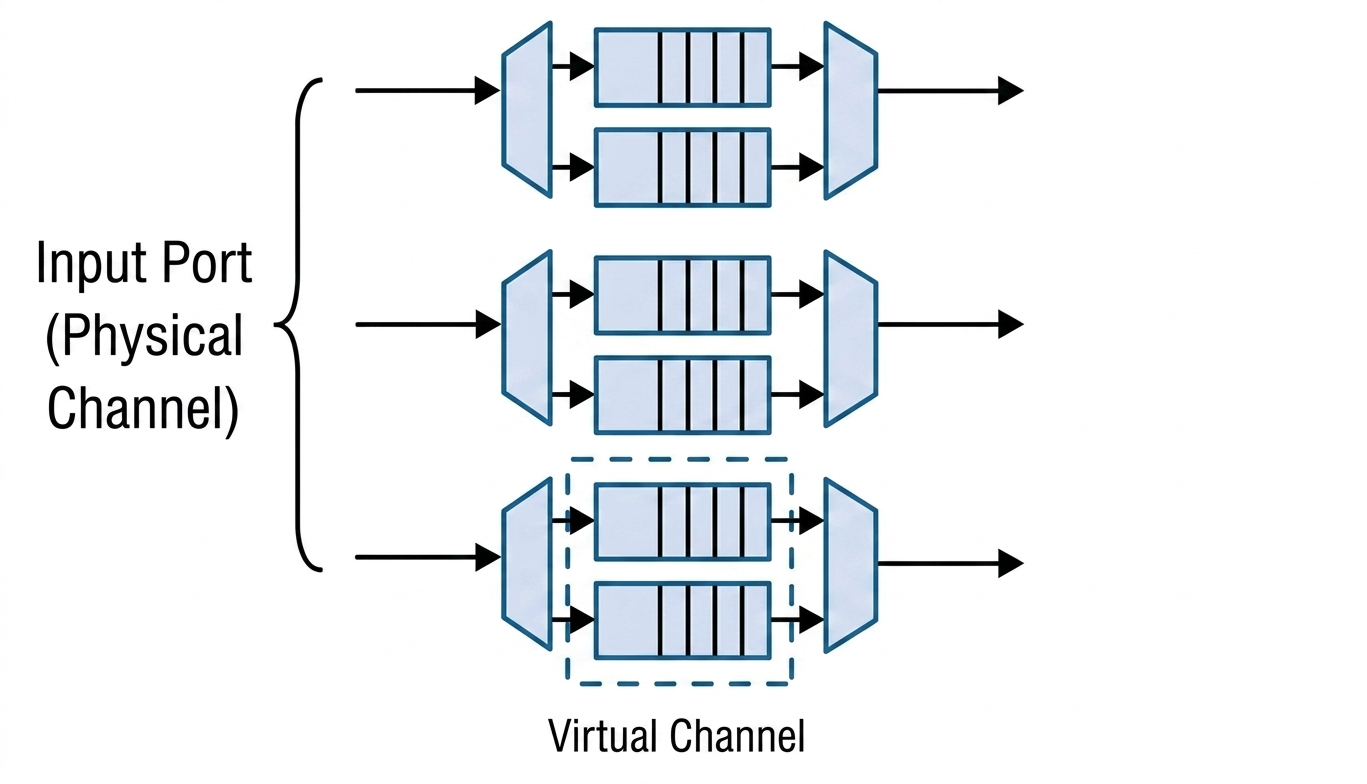
\includegraphics[width=0.6\textwidth]{images/ch2background/virtual_channel.png}
    \caption{Example of three Input Ports with two virtual channels per port}
    \label{fig:virtual_channel}
\end{figure}

At the input side of a router, incoming flits are stored in separate virtual-channel buffers and are later multiplexed onto the output link. If one packet is blocked in a certain virtual channel, packets belonging to other virtual channels may still continue to use the same physical channel. Therefore, virtual channels improve link utilization and reduce the blocking effect caused by resource contention.

Another important benefit of virtual channels is the reduction of head-of-line (HoL) blocking. Without virtual channels, a blocked packet at the front of a queue may prevent all following packets from moving forward, even if their desired paths are available. By separating packets into different virtual channels, this unnecessary blocking can be reduced, which improves overall network throughput and latency.

Virtual channels are also commonly used to support deadlock avoidance in NoC design. By assigning packets to different channel classes, cyclic resource dependencies can be reduced or eliminated. However, these benefits come at the cost of additional buffers, control logic, and allocation complexity in the router design.